%% LyX 2.4.2.1 created this file.  For more info, see https://www.lyx.org/.
%% Do not edit unless you really know what you are doing.
\documentclass[fontsize=12,ngerman,a4paper]{scrreprt}
\usepackage[T1]{fontenc}
\usepackage[utf8]{inputenc}
\setcounter{tocdepth}{3}
\usepackage{xcolor}
\usepackage{babel}
\usepackage{cprotect}
\usepackage{longtable}
\usepackage{calc}
\usepackage{url}
\usepackage{amsmath}
\usepackage{amssymb}
\usepackage{graphicx}
\usepackage[a4paper]{geometry}
\geometry{verbose,tmargin=0cm,bmargin=0cm,lmargin=0cm,rmargin=0cm,headheight=0cm,headsep=0cm,footskip=0cm}
\usepackage{rotating}
\usepackage{wasysym}
\usepackage[pdfusetitle,
 bookmarks=false,
 breaklinks=true,pdfborder={0 0 1},backref=false,colorlinks=true]
 {hyperref}

\makeatletter

%%%%%%%%%%%%%%%%%%%%%%%%%%%%%% LyX specific LaTeX commands.
%% Because html converters don't know tabularnewline
\providecommand{\tabularnewline}{\\}

%%%%%%%%%%%%%%%%%%%%%%%%%%%%%% User specified LaTeX commands.
\usepackage{tikz}
\usepackage{tikzpagenodes} 
\usepackage{palatino}
\usepackage{mathpazo}
\usepackage{upgreek}
\usepackage{datetime}
\usepackage{graphicx}
\usepackage{svn-multi}
\usepackage[absolute]{textpos}
\setlength{\parskip}{0mm}%
\setlength{\belowdisplayskip}{0pt}%
\setlength{\belowdisplayshortskip}{0pt}%
\setlength{\abovedisplayskip}{0pt}%
\setlength{\abovedisplayshortskip}{0pt}%
\setlength{\parindent}{0mm}
\newgeometry{left=1mm,bottom=1mm,top=1mm,right=1mm}
\usepackage{longtable}
\usepackage{multicol}
\usepackage{lipsum}

\usepackage{color}
\usepackage{blindtext}
\usepackage{tikz}
\urlstyle{rm}
\usepackage{capt-of}
\let\originalleft\left
\let\originalright\right
\renewcommand{\left}{\mathopen{}%
\mathclose\bgroup\originalleft}
\renewcommand{\right}{\aftergroup%
\egroup\originalright}
\usepackage[explicit]{titlesec}
%\titleformat{\section}{\bfseries}{}{0em}{BW.\thesection #1}%   \textbf ist ein makro und geht nicht
%\titleformat{\chapter}[display]{\scshape\bfseries\Large}{}{0mm}{\stepcounter{chapter}\thechapter\ #1}{}
%titleformat chapter... erfordert, secnumdepth!=-1.
\titleformat{\chapter}{\scshape\bfseries\Large}{}{0mm}{\thechapter\  #1} 
\titleformat{name=\chapter,numberless}{\scshape\bfseries\Large}{}{0mm}{#1}
\titleformat{\section}[runin]{\itshape\bfseries\large}{}{0mm}{\thesection\  #1}  %\vspace*{2pt}
\titleformat{name=\section,numberless}[runin]{\itshape\bfseries\large}{}{0mm}{#1} % \vspace*{2pt}
\titleformat{\subsection}[runin]{\itshape\bfseries\vspace*{2pt}}{}{0mm}{\thesection\  #1} 
\titleformat{name=\subsection,numberless}[runin]{\itshape\bfseries\vspace*{2pt}}{}{0mm}{#1}
\titlespacing*{\chapter}{0pt}{-7mm}{0pt}
\titlespacing*{\section}{0pt}{-2pt}{4pt} % Abstand {links}{drüber}{rechts}
\titlespacing*{\subsection}{0pt}{-2pt}{4pt}% Abstand {links}{drüber}{rechts}

\setcounter{section}{3}
\usepackage{booktabs}
\usepackage{enumitem}
\setlist[itemize,1]{leftmargin=\dimexpr 5mm, topsep=0mm} % Veraendert den Abstand vor Aufzaehlungspunkten
\setlist[itemize,2]{leftmargin=\dimexpr 5mm, topsep=0mm} % Veraendert den Abstand vor Aufzaehlungspunkten
\setlist[enumerate,1]{leftmargin=\dimexpr 8mm, topsep=0mm, parsep=0mm, itemsep=0mm} % Veraendert den Abstand vor Aufzaehlungspunkten
\setlist[enumerate,2]{leftmargin=\dimexpr 8mm, topsep=0mm, parsep=0mm, itemsep=0mm} % Veraendert den Abstand vor Aufzaehlungspunkten

\mathcode `,="013B
\mathcode `.="613A
\DeclareMathAlphabet{\mathbfit}{OML}{cmm}{b}{it}
\makeatletter
% Der nachfolgende Befehl erfordert das Paket amsmath
\newcommand{\eqnum}{\refstepcounter{equation}\textup{\tagform@{\theequation}}}
\makeatother
\renewcommand{\theequation}{\ifnum\thechapter=666 FS\else \thechapter\fi .\arabic{equation}}
\renewcommand{\thetable}{\ifnum\thechapter=666 FS\else \thechapter\fi .\arabic{table}}
\makeatletter
\DeclareMathSizes{\@xpt}{\@xpt}{\@xpt}{\@xpt}
\makeatother
\DeclareMathSizes{10.95}{11}{13}{13}
\def\tsrotate{90}

\usepackage[type={CC},modifier={by},version={4.0},]{doclicense}
\renewcommand{\UrlBreaks}{\do\/ %
\do\a\do\b\do\c\do\d\do\e\do\f\do\g\do\h\do\i\do\j\do\k\do\l % 
\do\m\do\n\do\o\do\p\do\q\do\r\do\s\do\t\do\u\do\v\do\w\do\x %
\do\y\do\z\do\A\do\B\do\C\do\D\do\E\do\F\do\G\do\H\do\I\do\J %
\do\K\do\L\do\M\do\N\do\O\do\P\do\Q\do\R\do\S\do\T\do\U\do\V %
\do\W\do\X\do\Y\do\Z}

\makeatother

\usepackage{listings}
\lstset{numberstyle={\tiny},
numbersep=0pt,
basicstyle={\ttfamily},
breaklines=true}
\renewcommand{\lstlistingname}{\inputencoding{latin9}Listing}

\begin{document}
\newcommand{\ueberschrift}{\LaTeX -Cheat Sheet template, \\Author: Prof. Dr. Thorbjörn Siaenen}

\providecommand\tssection[1]{
\tikz{ \node[draw] (0,0){sdf}; }
}
\thispagestyle{empty}%
% maximal print width on a Brother 8510DN is 196 mm
% left and right have to be 7 mm margins, above and below 4.5 mm (better: 5 mm)
\setlength\abovedisplayskip{0pt}
\setlength\belowdisplayskip{0pt}
\setlength\abovedisplayshortskip{0pt}
\setlength\belowdisplayshortskip{0pt}
% Distances in a Bullet-Point-List:
\let\tempone\itemize
\let\temptwo\enditemize
\renewenvironment{itemize}{\tempone\setlength{\itemsep}{1pt} \setlength{\parskip}{0pt}}{\temptwo}

\ifx\tsrechts\undefined
\newlength{\tsrechts}
\setlength{\tsrechts}{6mm}
\fi
\ifx\tsoben\undefined
\newlength{\tsoben}
\setlength{\tsoben}{0mm}
\fi
\ifdefined \tsscalefactor \else
\newcommand{\tsscalefactor}{0.99}
\fi
\vspace*{\tsoben} %
\thispagestyle{plain}%

\hspace*{\tsrechts}\begin{tikzpicture}[inner sep=1pt, scale=\tsscalefactor]%
%inner sep = abstand zwischen Rand und Inhalt-Nodes

\draw[line width=0.5*\tsscalefactor] (0,0) rectangle (196mm,287mm);
\fill[gray] (3mm,183.5mm) circle (3mm);
\fill[gray] (3mm,103.5mm) circle (3mm);
\draw[line width=0.5*\tsscalefactor] (0,47.833mm) -- (196mm,47.833mm);
\draw[line width=0.5*\tsscalefactor] (0,95.666mm) -- (196mm,95.666mm);
\draw[line width=0.5*\tsscalefactor] (10mm,143.5mm) -- (196mm,143.5mm);
\draw[line width=0.5*\tsscalefactor] (0,191.33mm) -- (196mm,191.33mm);
\draw[line width=0.5*\tsscalefactor] (0,239.166mm) -- (196mm,239.166mm);
\draw[line width=0.5*\tsscalefactor] (0.5mm,143.5mm) node[scale=0.6*\tsscalefactor, text width=140mm, align=center, anchor = north,rotate=90,inner sep=0mm]{\sffamily\textbf{\ueberschrift}};

%Erste Spalte:
%ampersand replacement = \tseqseparator ist wichtig, wenn in dem node eine Tabelle stehen soll
\matrix[row sep=0mm, column sep = 0pt, matrix anchor=west,ampersand replacement=\tseqseparator] at (0,23.91666mm){

\setlength{\itemindent}{0em}

\node[rotate=\tsrotate, inner sep=2pt, scale=0.49*\tsscalefactor,text width=94mm, draw, line width=0.5*\tsscalefactor]{\doclicenseThis %
};\tseqseparator

\node[rotate=\tsrotate, inner sep=2pt, scale=0.49*\tsscalefactor,text width=94mm, draw, line width=0.5*\tsscalefactor]{
\chapter{Allgemeines}%
};\tseqseparator

\node[rotate=\tsrotate, inner sep=2pt, scale=0.49*\tsscalefactor,text width=94mm, draw, line width=0.5*\tsscalefactor]{
\section{Einleitung}

Diese Vorlage einer Formelsammlung kann dazu verwendet werden eine
beliebige Formelsammlung zu erstellen. Diese Formelsammlung hat die
folgenden Eigenschaften: Sie wird mit LaTeX erstellt (eine LyX-Datei
ist ebenfalls verfügbar). Die Schriftgröße ist 6. Das ist klein genug,
dass viel Inhalt auf eine Seite passt und groß genug um noch gelesen
werden zu können. Indizes und Exponenten werden nicht in kleinerer
Schriftart gesetzt. Damit bleibt die Lesbarkeit erhalten. Es sind
viele Beispiele für Formelsammlungselemente enthalten (Formeln, Tabellen,
Bilder, Aufzählungen u.s.w). Sollte etwas fehlen oder es ihnen gefallen,
schreiben Sie an

\hspace*{\fill}\textcolor{blue}{\href{mailto:t.siaenen@ostfalia.de}{t.siaenen@ostfalia.de}}\hspace*{\fill}~%
};\tseqseparator

\node[rotate=\tsrotate, inner sep=2pt, scale=0.49*\tsscalefactor,text width=94mm, draw, line width=0.5*\tsscalefactor]{
\section{Technisches in Bezug auf LaTeX}

\label{eq:formelnr1}Sie ist mit dem Programm mit LaTeX erstellt.
LaTeX ist eine Beschreibungssprache für Dokumente. Das Dokument wird
mit verschiedenen Befehlen beschrieben und der beschreibende Text
in einer Text-Datei gespeichert. Diese Text-Datei wird in eine PDF-Datei
umgewandelt, wobei viele Befehle dazu führen, dass Tabellen, Formeln,
Abbildungen und Aufzählungen formschön gesetzt werden.

Unter Windows lautet der Befehl zum Umwandeln: \texttt{pdflatex UniversalFormelsammlung.tex}. 

Dies setzt voraus, dass (unter Windows) das Programm MikTex (\url{www.miktex.org})
installiert ist. Als Editor wird notepad++ oder texmaker empfohlen.
Dieses Dokument ist keine abschließende Schulung in dem System LaTeX,
sondern soll Sie lediglich in die Lage versetzten eine Formelsammlung
zu erstellen. Für umfassendere Informationen werden die Unterlagen
der Fernuni-Hagen empfohlen: \url{https://www.fernuni-hagen.de/zdi/docs/a026_latex_einf.pdf} %
};\tseqseparator

\node[rotate=\tsrotate, inner sep=2pt, scale=0.49*\tsscalefactor,text width=94mm, draw, line width=0.5*\tsscalefactor]{
\section{Technisches in Bezug auf LyX}

\label{eq:technischeslyx}Die LyX-Vorlage verwendet zwei Module, die
vor der Benutzung installiert werden müssen. Die Datei \texttt{formelsammlungnode\_v6.module}
wird in das Verzeichnis ,,C:\textbackslash Users\textbackslash BENUTZERNAME\textbackslash AppData\textbackslash\-Roa\-ming\textbackslash LyX2.3\textbackslash layouts''
(in früheren LyX-Versionen ,,C:\textbackslash Program Files (x86)\textbackslash LyX
2.3\textbackslash Resources\textbackslash layouts'') kopiert. Weiterhin
muss in LyX die Befehlsfolge ,,Werkzeuge -> neu Konfigurieren''
ausgeführt werden.

In den Spalten stehen dann untereinander Blöcke des Typs ,,Formel''.
Der letzte Block innerhalb einer Spalte muss vom Typ ,,letzte Formel''
sein.%
};\\};

%Zweite Spalte:
\matrix[row sep=0mm, column sep = 0pt, matrix anchor=west,ampersand replacement=\tseqseparator] at (0,71.749995mm){

\node[rotate=\tsrotate, inner sep=2pt, scale=0.49*\tsscalefactor,text width=94mm, draw, line width=0.5*\tsscalefactor]{
\section{Eigenschaften dieser Formelsammlung}

\label{eq:eigenschaftenformelsammlung}
\begin{itemize}
\item Sie ist mit dem Computer erstellt
\begin{itemize}
\item Änderungen, Umsortieren und Korrekturen sind Rückstandsfrei möglich
\item Man lernt, besser mit dem Computer umzugehen
\end{itemize}
\item Druckränder des Druckers sind berücksichtigt
\item Es passt ein Maximum an Inhalt auf eine Seite: Bei der Schriftgröße
wurde ein Kompromiss aus Informationsdichte und Lesbarkeit getroffen.
\item Die Schriftgröße von Indizes wird nicht verkleinert.
\item Tabelle, Grafiken, Aufzählungen, Auflistungen und Formeln sind exemplarisch
gezeigt.
\item Aufteilung in Kapitel, Abschnitte und Unterabschnitte ermöglichen
die Klassifizierung des Inhaltes.
\end{itemize}
Hinweis: Eine gute Formelsammlung ist sicherlich schneller kopiert
als selbst erstellt. Es ist besser, eine Formelsammlung selbst zu
erstellen. Das eigenständige Reflektieren und Zusammenfassen von Lehrinhalten
ist ein wesentlicher Bestandteil des Lernprozesses. Dieser wird übersprungen,
wenn beispielsweise eine Formelsammlung kopiert wird, anstatt sie
selbst zu erstellen.%
};\tseqseparator

\node[rotate=\tsrotate, inner sep=2pt, scale=0.49*\tsscalefactor,text width=94mm, draw, line width=0.5*\tsscalefactor]{
\chapter{Beispielelemente }%
};\tseqseparator

\node[rotate=\tsrotate, inner sep=2pt, scale=0.49*\tsscalefactor,text width=94mm, draw, line width=0.5*\tsscalefactor]{
\section{Elemente mit Rahmen}

\noindent\fcolorbox{black}{white}{\begin{minipage}[t]{1\columnwidth - 2\fboxsep - 2\fboxrule}%
Dies ist eine Formel $x^{2}+y^{2}=z^{2}$ in einem Kästchen \hfill{}\eqnum\label{eq:formelinkaestchen}%
\end{minipage}}

\noindent\fcolorbox{black}{white}{\begin{minipage}[t]{1\columnwidth - 2\fboxsep - 2\fboxrule}%
Dies ist eine Formel $\mathrm{e^{\mathrm{j}\,\pi}}+1=0$ in einem
Kästchen \hfill{}\eqnum\label{eq:formelinkaestchenzwei}%
\end{minipage}}

Dies ist ein Text unterhalb der Kästchen.\hfill{}\eqnum\label{eq:kaestchenmitrahmen}%
};\tseqseparator

\node[rotate=\tsrotate, inner sep=2pt, scale=0.49*\tsscalefactor,text width=94mm, draw, line width=0.5*\tsscalefactor]{
\section{Farben}

\label{sec:farben}Der Text kann in verschiedene Farben gesetzt werden.
Diese sind \textcolor{blue}{Blau}, \textcolor{teal}{Blaugrün}, \textcolor{brown}{Braun},
\textcolor{cyan}{Cyan}, \textcolor{darkgray}{Dunkelgrau}, \textcolor{yellow}{Gelb},
\textcolor{gray}{Grau}, \textcolor{green}{Grün}, \textcolor{lightgray}{Hellgrau},
\textcolor{magenta}{Magenta}, \textcolor{lime}{Neongrün}, \textcolor{olive}{Olivgrün},
\textcolor{orange}{Orange}, \textcolor{pink}{Pink}, \textcolor{purple}{Purpur},
\textcolor{red}{Rot}, \textcolor{black}{Schwarz}, \textcolor{violet}{Violett}
und {\rlap{\raisebox{-0.4mm}{\rule{11mm}{4.4mm}}}\textcolor{white}{\hspace*{0.3mm}Weiß.}}

Wenn Farbdefinitionen verschachtelt sind, dann wird der Text in der
innersten verschachtelten Farbe gesetzt: \textcolor{blue}{Blauer Text, \textcolor{orange}{orangener Text}, blauer Text}%
};\tseqseparator

\node[rotate=\tsrotate, inner sep=2pt, scale=0.49*\tsscalefactor,text width=94mm, draw, line width=0.5*\tsscalefactor]{
\section{Aufzählungen}

\label{eq:aufzaehlung}Ein weiteres Element ist die Aufzählung:
\begin{enumerate}
\item Erstes Element
\item Zweites Element
\begin{enumerate}
\item Zweites Element, Teil a
\item Zweites Element, Teil b
\end{enumerate}
\item Drittes Element
\end{enumerate}
%
};\tseqseparator

\node[rotate=\tsrotate, inner sep=2pt, scale=0.49*\tsscalefactor,text width=94mm, draw, line width=0.5*\tsscalefactor]{
\section{Stichpunkte}

\label{eq:aufzaehlung2}Ein weiteres Element ist die Aufzählung:
\begin{itemize}
\item Erstes Elemen
\item Zweites Element
\begin{itemize}
\item Zweites Element, Teil a
\item Zweites Element, Teil b
\end{itemize}
\item Drittes Element
\end{itemize}
%
};\\};

%Dritte Spalte:
\matrix[row sep=0mm, column sep = 0pt, matrix anchor=west,ampersand replacement=\tseqseparator] at (6.5mm,119.583325mm){

\node[rotate=\tsrotate, inner sep=2pt, scale=0.49*\tsscalefactor,text width=94mm, draw, line width=0.5*\tsscalefactor]{
\section{Tabellen}

\label{eq:tabellengestaltung}~\newline

\hfill{}%
\begin{tabular}{|c|c|c|c|}
\hline 
\begin{turn}{90}
Überschrift
\end{turn} & \begin{turn}{90}
Überschrift
\end{turn} & \begin{turn}{90}
Überschrift
\end{turn} & \begin{turn}{90}
Überschrift
\end{turn}\tabularnewline
\hline 
\hline 
1 & 2 & 3 & 4\tabularnewline
\hline 
$x^{2}$ & $x^{3}$ & $x^{4}$ & $x^{5}$\tabularnewline
\hline 
a & b & c & d\tabularnewline
\hline 
\end{tabular}\hfill{}\null%
\begin{longtable}[c]{|r|c|}
\caption{Ausrichtung am Komma \label{tab:komma}}
\tabularnewline
\hline 
\textbf{Station}  & \textbf{Messwert~(V)}\tabularnewline
\endfirsthead
\hline 
4711  & \hphantom{000}3,14\hphantom{0} \tabularnewline
\hline 
0815  & \phantom{000}2,74\hphantom{0} \tabularnewline
\hline 
0123456789  & \hphantom{000}2,345 \tabularnewline
\hline 
0123456  & \hphantom{00}12,3\hphantom{00} \tabularnewline
\hline 
007  & 2345,3\hphantom{00} \tabularnewline
\hline 
\end{longtable}%
};\tseqseparator

\node[rotate=\tsrotate, inner sep=2pt, scale=0.49*\tsscalefactor,text width=94mm, draw, line width=0.5*\tsscalefactor]{
\chapter{Unterteilungen}%
};\tseqseparator

\node[rotate=\tsrotate, inner sep=2pt, scale=0.49*\tsscalefactor,text width=94mm, draw, line width=0.5*\tsscalefactor]{
\section{Kästchen}

\label{eq:unerteilungen}Texte können noch unterteilt werden:

\section{Abschnittsüberschrift}

Dies ist die erste Zeile in diesem Abschnitt. Es folgen zwei Unter-Abschnitte

\subsection{Unterabschnitt A}

Dies ist eine Zeile Text im Unterabschnitt A

\subsection{Unterabschnitt B}

Dies ist eine Zeile Text im Unterabschnitt B%
};\tseqseparator

\node[rotate=\tsrotate, inner sep=2pt, scale=0.49*\tsscalefactor,text width=94mm, draw, line width=0.5*\tsscalefactor]{
\section{Zeilenumbruch nach Überschrift}

~\\Hier ist gezeigt, wie nach der Überschrift künstlich ein Zeilenumbruch
eingebaut werden kann.

\section{Horizontale Linie}

Weiterhin ist hier ein Beispel für eine horizontale Linie über die
Breite einer Spalte:

\hrulefill~\\

Und hier ist noch mehr Text.%
};\tseqseparator

\node[rotate=\tsrotate, inner sep=2pt, scale=0.49*\tsscalefactor,text width=94mm, draw, line width=0.5*\tsscalefactor]{
\section{Zeilenumbruch nach Überschrift}

~\\Hier ist gezeigt, wie nach der Überschrift künstlich ein Zeilenumbruch
eingebaut werden kann.

\section{Horizontale Linie}

Weiterhin ist hier ein Beispel für eine horizontale Linie über die
Breite einer Spalte:

\hrulefill~\\

Und hier ist noch mehr Text.%
};\tseqseparator

\node[rotate=\tsrotate, inner sep=2pt, scale=0.49*\tsscalefactor,text width=94mm, draw, line width=0.5*\tsscalefactor]{
\section{Fließtext und Formeln}

\label{eq:formelnnummeriert}Formeln können in zwei Varianten geschrieben
stehen: Einmal im Text: $\mathrm{sin}(x)=\pi/3$ wie in diesem Beispiel,
oder als abgesetzte Formel: 
\[
\mathrm{sin}(x)=\pi/3
\]
Weiterhin kann man eine Formel auch automatisch nummerieren lassen:
\begin{equation}
\mathrm{sin}(x)=\pi/3\label{eq:abgesetzteformel}
\end{equation}
In dem Text kann dann auf die Gleichung (\ref{eq:abgesetzteformel})
(Achtung: Das Paket hyperref erzeugt Hyperlinks die auf der Seite
an falscher Position liegen) referenziert werden. Zwei Abgesetzte
Formeln nebeneinander können mit folgender Struktur dargestellt werden:

\begin{minipage}[t]{0.39\textwidth}%
\begin{equation}
\mathrm{e}^{\mathrm{j\,\pi}}+1=0\label{eq:allekonstentenineinergleichung}
\end{equation}
%
\end{minipage} %
\begin{minipage}[t]{0.59\textwidth}%
\begin{equation}
\mathrm{sin}(x)^{2}+\mathrm{cos}(x)^{2}=1\label{eq:trigonometrischerpythagora}
\end{equation}
%
\end{minipage} 

Alternative Darstellungsweise mit Kästchen: 

\fcolorbox{black}{white}{\begin{minipage}[t]{0.38\textwidth}%
\begin{equation}
\mathrm{e}^{\mathrm{j\,\pi}}+1=0\label{eq:allekonstentenineinergleichung-1}
\end{equation}
%
\end{minipage}}%
\fcolorbox{black}{white}{\begin{minipage}[t]{0.57\textwidth}%
\begin{equation}
\mathrm{sin}(x)^{2}+\mathrm{cos}(x)^{2}=1\label{eq:trigonometrischerpythagora-1}
\end{equation}
%
\end{minipage}}

Wenn statt der Gleichungsnummer zwei Fragezeichen erscheinen muss
häufig die Datei noch einmal übersetzt, oder label und ref haben unterschiedliche
Marken. Beim Konvertieren zwischen der .TEX-Datei und der PDF-Datei
spricht man vom sog. \textit{Setzen}. %
};\\};

%vierte Spalte:
\matrix[row sep=0mm, column sep = 0pt, matrix anchor=west,ampersand replacement=\tseqseparator] at (6.5mm,167.416655mm){

\node[rotate=\tsrotate, inner sep=2pt, scale=0.49*\tsscalefactor,text width=94mm, draw, line width=0.5*\tsscalefactor]{
\section{Formelsatz}%
};\tseqseparator

\node[rotate=\tsrotate, inner sep=2pt, scale=0.49*\tsscalefactor,text width=94mm, draw, line width=0.5*\tsscalefactor]{
\section{Regeln zum Formelsatz}

\label{eq:formelsatz}Für das Setzen von Formeln gibt es Regeln:
\begin{itemize}
\item Variablen werden kursiv gesetzt
\item Indizes, Konstanten, physikalische Einheiten und Funktionsnamen werden
aufrecht gesetzt
\end{itemize}
Also: $x_{\mathrm{start}}$ statt $x_{start}$, $\mathrm{sin}(x)$
statt $sin(x)$, $z=4+\mathrm{j}\,6$ statt $z=4+j\,6$, $i=4{,}5\,\mathrm{A}$
statt $i=4{,}5\,A$ und $\mathrm{e}^{\mathrm{j}\,\pi}$ statt $e^{j\,\pi}$.
Bei Zahlenwerten in Formeln sollte das Komma als Dezimaltrennzeichen
in geschweifte Klammern gesetzt werden. Damit wird ein falscher Leerraum
verhindert. Richtig: $\pi=3{,}14$. Falsch: \raisebox{-1mm}{
\includegraphics[width=19mm]{figures/fig_kommaabstand/kommaabstand}}

In Formeln kommen beispielhaft folgende Elemente vor:
\begin{itemize}
\item Wurzel: $\sqrt{\left(x\right)}$
\item n-te Wurzel: $\sqrt[3]{x}$
\item Bruch: $\frac{\text{Zähler}}{\text{Nenner}}$
\item Index: $x_{1}$
\item Index mit mehreren Buchstaben: $x_{\mathrm{start}}$
\item Sub-(sub-)Indizes: $S_{v_{\mathrm{end}_{2}}}$
\item Exponent: $x^{2}$
\item Exponent mit mehreren Buchstaben: $x^{12}$
\item Integral: $\int x^{2}\,\mathrm{d}x$ 
\item Bestimmtes Integral: $\int_{0}^{\infty}f(x)\,\mathrm{d}x$
\item Buchstaben aufrecht gesetzt (nicht kursiv): $\mathrm{x}$
\item Summenzeichen: $\sum$
\item Summenzeichen mit Grenzen: $\sum_{k=1}^{42}$
\item Griechische Buchstaben: $\alpha$, $\beta$, $\gamma$, $\theta$
\item Multiplikationspunkt (nicht: \$a{*}b\$): $a\cdot b$
\item Geschweifte Klammern unten: $\underbrace{a\cdot b}_{c}$
\item Geschweifte Klammern oben: $\overbrace{0\cdot b}^{=0}$
\item Abstand: klein (Multiplikation) $a\,b$
\item Abstand: mittel $a\ b$
\item Abstand: groß $a\quad b$
\item Doppelter großer Abstand: $a\qquad b$
\item Man achte darauf, dass nach dem Mathebefehl ein Leerzeichen steht:
$\alpha a$ \% Hinweis: \$\textbackslash alphaa\$ funktioniert nicht
\item Klammern, deren Größe sich dem Inhalt anpassen: $\left[\sqrt{x^{2}}\right]$,
$\left(\sqrt{x^{2}}\right)$, 
\item $\left|\sqrt{x^{2}}\right|$ statt $[\sqrt{x^{2}}]$, $(\sqrt{x^{2}})$,
$|\sqrt{x^{2}}|$
\item Klammern und senkrechte Striche in unterschiedlicher Größe: $\bigr)$
$\biggr)$ $\Biggr)$ $\bigl($ $\biggl($ $\Biggl($ $\bigr]$ $\biggr]$
$\Biggr]$ $\bigl[$ $\biggl[$ $\Biggl[$ $\bigr|$ $\biggr|$ $\Biggr|$ 
\item Matrix: $\left(\begin{matrix}11 & 12\\
21 & 22
\end{matrix}\right)$
\item Limes: $\lim_{x\rightarrow\infty}$ oder ${\displaystyle \lim_{x\rightarrow\infty}}$
\end{itemize}
(Fortführung in der nächsten Spalte...)%
};\\};

%fünfte Spalte:
\matrix[row sep=0mm, column sep = 0pt, matrix anchor=west,ampersand replacement=\tseqseparator] at (0mm,215.249985mm){

\node[rotate=\tsrotate, inner sep=2pt, scale=0.49*\tsscalefactor,text width=94mm, draw, line width=0.5*\tsscalefactor]{
\section{Regeln zum Formelsatz (Fortführung)}

\label{eq:formelsatz-2}
\begin{itemize}
\item Geschweifte Klammer unterhalb: $\underbrace{1+2+3}_{=6}+4$
\item Geschweifte Klammer oberhalb: $1+\overbrace{2+3+4}^{=9}$
\item Strich unterhalb: $\underline{z}$
\item Teile von Formeln können auch in unterschiedlichen Farben gesetzt
werden:$\mathop{\color{blue}\sin}{\color{blue}\left({\color{brown}x}\right)^{2}+\mathop{\color{magenta}\cos}}\left(x\right)^{2}={\color{green}1}$
\item Sonderzeichen: $\smiley$
\end{itemize}
Je nach Umgebung (in-Zeile-Formel oder abgesetzte Formel) werden einige
Elemente in unterschiedlicher Größe dargestellt:$\int_{0}^{\infty}\mathrm{sin}(x)\,\mathrm{d}x$
\[
\int_{0}^{\infty}\mathrm{sin}(x)\,\mathrm{d}x
\]
In-Zeile-Formeln können in der Größe von abgesetzten Formeln gesetzt
werden: ${\displaystyle {\displaystyle \int_{0}^{\infty}\mathrm{sin}(x)\,\mathrm{d}x}}$

Latex kennt eine Vielzahl an Sonderzeichen: Erkennung von Sonderzeichen:
\url{http://detexify.kirelabs.org/classify.html} Übersicht der Sonderzeichen:
\url{http://mirrors.ctan.org/info/symbols/comprehensive/symbols-a4.pdf}%
};\tseqseparator

\node[rotate=\tsrotate, inner sep=2pt, scale=0.49*\tsscalefactor,text width=94mm, draw, line width=0.5*\tsscalefactor]{
\chapter{Abbildungen}%
};\tseqseparator

\node[rotate=\tsrotate, inner sep=2pt, scale=0.49*\tsscalefactor,text width=94mm, draw, line width=0.5*\tsscalefactor]{
\section{Abbildungen}

\label{eq:abbildungen}Beispiel:

\hfill{}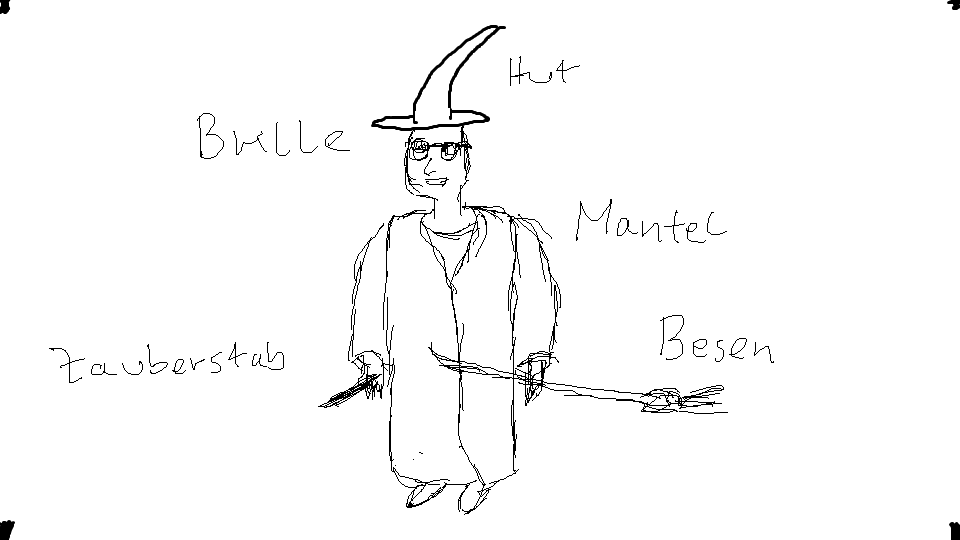
\includegraphics[width=90mm]{figures/fig_zauberer/zauberer}\hfill{}

Abbildung 1: Eine Abbildung über eine Spalte

\hfill{}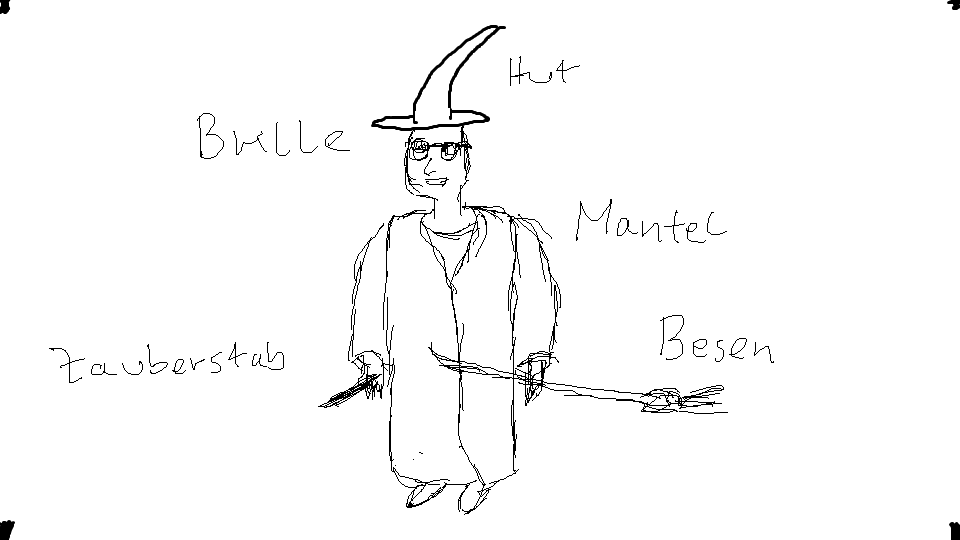
\includegraphics[width=45mm]{figures/fig_zauberer/zauberer}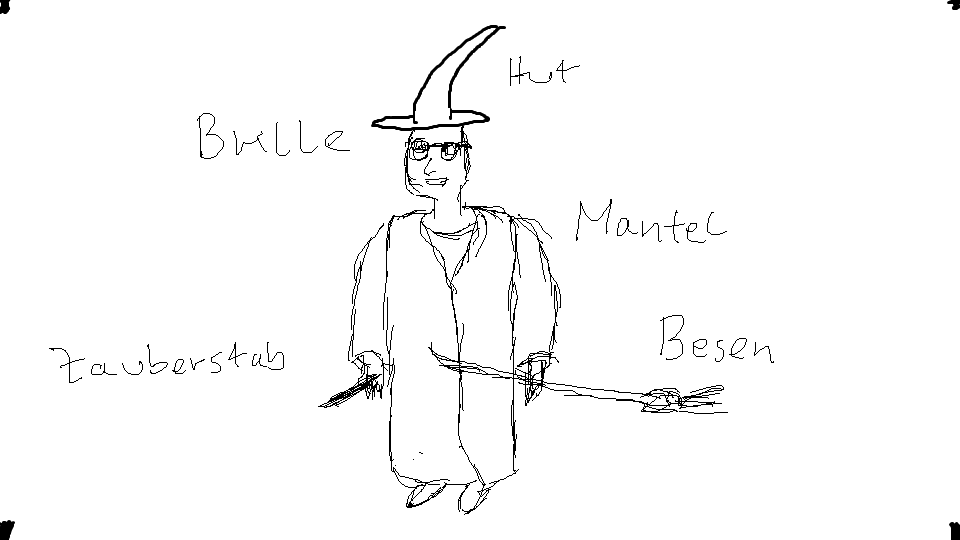
\includegraphics[width=45mm]{figures/fig_zauberer/zauberer}\hfill{}

\hfill{}Halbe Seitenbreite\hfill{}\hfill{}Halbe Seitenbreite\hfill{}

Abbildung gedreht:

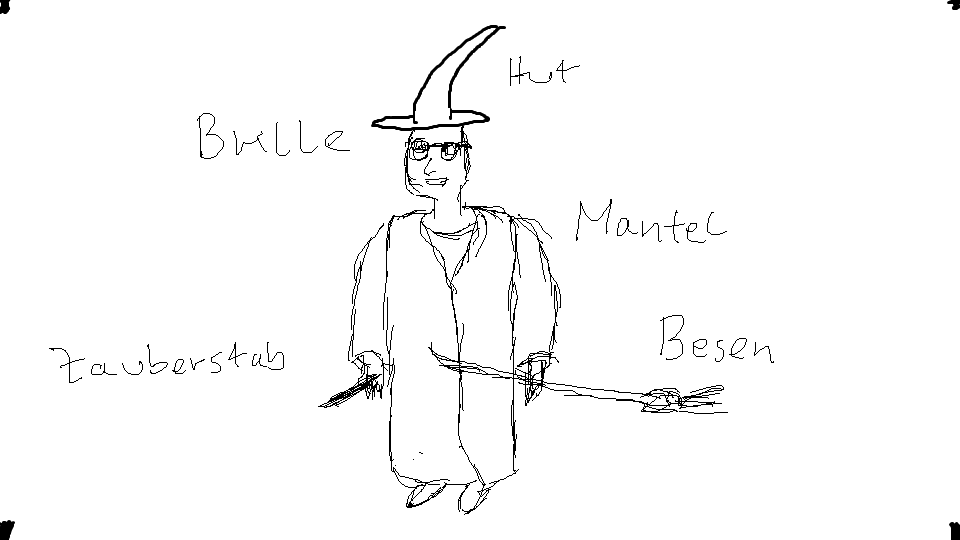
\includegraphics[angle=90,width=90mm]{figures/fig_zauberer/zauberer}%
};\\};

%sechste Spalte:
\matrix[row sep=0mm, column sep = 0pt, matrix anchor=west,ampersand replacement=\tseqseparator] at (0mm,263.083315mm){

\node[rotate=\tsrotate, inner sep=2pt, scale=0.49*\tsscalefactor,text width=94mm, draw, line width=0.5*\tsscalefactor]{
\chapter{Sechste Spalte}%
};\tseqseparator

\node[rotate=\tsrotate, inner sep=2pt, scale=0.49*\tsscalefactor,text width=94mm, draw, line width=0.5*\tsscalefactor]{{\Large\textsf{\textbf{\textit{$\blacksquare$}}}}{\large\textbf{\textit{Formeln
verkleinern}}}{\large\par}

Manchmal sind Formeln so breit, dass sie nicht in eine Zeile hineinpassen.
In einigen Fällen kann durch ,,quetschen'' soviel Platz eingespart
werden, dass die Formel doch in eine Zeile passt. Dies erfolgt durch
Einfügen von ,,negativen Abständen''. Beispiel einer zu breiten
Formel:
\[
\left(\begin{array}{c}
u_{\mathrm{L1}}\\
u_{\mathrm{L2}}\\
1
\end{array}\right)=\left(\left(\begin{array}{c}
u_{10}\\
u_{20}\\
1
\end{array}\right)\cdot\left(\begin{array}{ccc}
1 & 1 & 1\end{array}\right)+\left(\begin{array}{ccc}
\frac{1}{3} & \frac{1}{3} & \frac{2}{3}\\
\frac{1}{3} & \frac{-2}{3} & \frac{-1}{3}\\
0 & 0 & 0
\end{array}\right)\,u_{\mathrm{C}}\right)\cdot\left(\begin{array}{c}
k_{1}\\
k_{2}\\
k_{3}
\end{array}\right)
\]

Abhilfe:

\[
\negmedspace\left(\negmedspace\negmedspace\negmedspace\begin{array}{c}
u_{\mathrm{L1}}\\
u_{\mathrm{L2}}\\
1
\end{array}\negmedspace\negmedspace\negmedspace\right)\negmedspace=\negmedspace\left(\negmedspace\negmedspace\negmedspace\left(\negmedspace\negmedspace\negmedspace\begin{array}{c}
u_{10}\\
u_{20}\\
1
\end{array}\negmedspace\negmedspace\negmedspace\right)\negmedspace\cdot\negmedspace\left(\negmedspace\negmedspace\begin{array}{ccc}
\negmedspace1\negmedspace & \negmedspace1\negmedspace & \negmedspace1\negmedspace\end{array}\negmedspace\negmedspace\right)\negmedspace+\negmedspace\left(\negmedspace\negmedspace\begin{array}{ccc}
\frac{1}{3} & \frac{1}{3} & \frac{2}{3}\\
\frac{1}{3} & \frac{-2}{3} & \frac{-1}{3}\\
0 & 0 & 0
\end{array}\negmedspace\negmedspace\negmedspace\right)\,u_{\mathrm{C}}\negmedspace\negmedspace\right)\negmedspace\cdot\negmedspace\left(\negmedspace\negmedspace\negmedspace\begin{array}{c}
k_{1}\\
k_{2}\\
k_{3}
\end{array}\negmedspace\negmedspace\negmedspace\right)
\]

Abhilfe durch Umbrüche:

\begin{multline*}
\left(\begin{array}{c}
u_{\mathrm{L1}}\\
u_{\mathrm{L2}}\\
1
\end{array}\right)=\Biggl(\left(\begin{array}{c}
u_{10}\\
u_{20}\\
1
\end{array}\right)\cdot\left(\begin{array}{ccc}
1 & 1 & 1\end{array}\right)+\\
\left(\begin{array}{ccc}
\frac{1}{3} & \frac{1}{3} & \frac{2}{3}\\
\frac{1}{3} & \frac{-2}{3} & \frac{-1}{3}\\
0 & 0 & 0
\end{array}\right)\,u_{\mathrm{C}}\Biggr)\cdot\left(\begin{array}{c}
k_{1}\\
k_{2}\\
k_{3}
\end{array}\right)
\end{multline*}

Hinweis: Klammergruppen mit \texttt{\textbackslash left(} und \texttt{\textbackslash right)}
können nicht mit einem Umbruch versehen werden. Abhilfe schafft eine
manuelle Größeneinstellung einer Klammer mit beispielsweise \texttt{\textbackslash Biggl(}
und \texttt{\textbackslash Biggr)}.

\hfill{}\eqnum\label{eq:formelsatz-1}%
};\tseqseparator

\node[rotate=\tsrotate, inner sep=2pt, scale=0.49*\tsscalefactor,text width=94mm, draw, line width=0.5*\tsscalefactor]{
\section{Source-Code}

\label{sec:sourcecode}Source-Code kann mit einer sog. Listings-Umgebung
gesetzt werden:

\bgroup\inputencoding{latin9}
\begin{lstlisting}
Dies ist ein Source-Code mit einer sehr sehr sehr langen Zeile, die automatisch umbebrochen wird.
\end{lstlisting}
\leavevmode\egroup
%
};\\};

\end{tikzpicture}%

\newpage{}

\vspace*{1mm} %
\thispagestyle{plain}%
\hspace*{\tsrechts}\begin{tikzpicture}[inner sep=1pt, scale=\tsscalefactor]%
%inner sep = abstand zwischen Rand und Inhalt-Nodes

\draw[line width=0.5*\tsscalefactor] (0,0) rectangle (196mm,287mm);
\fill[gray] (3mm,183.5mm) circle (3mm);
\fill[gray] (3mm,103.5mm) circle (3mm);
\draw[line width=0.5*\tsscalefactor] (0,47.833mm) -- (196mm,47.833mm);
\draw[line width=0.5*\tsscalefactor] (0,95.666mm) -- (196mm,95.666mm);
\draw[line width=0.5*\tsscalefactor] (10mm,143.5mm) -- (196mm,143.5mm);
\draw[line width=0.5*\tsscalefactor] (0,191.33mm) -- (196mm,191.33mm);
\draw[line width=0.5*\tsscalefactor] (0,239.166mm) -- (196mm,239.166mm);
\draw[line width=0.5*\tsscalefactor] (0.5mm,143.5mm) node[scale=0.6*\tsscalefactor, text width=140mm, align=center, anchor = north,rotate=90,inner sep=0mm]{\sffamily\textbf{\ueberschrift}};

%Erste Spalte:
%ampersand replacement = \& ist wichtig, wenn in dem node eine Tabelle stehen soll
\matrix[row sep=0mm, column sep = 0pt, matrix anchor=west,ampersand replacement=\tseqseparator] at (0,23.91666mm){

\node[rotate=\tsrotate, inner sep=2pt, scale=0.49*\tsscalefactor,text width=94mm, draw, line width=0.5*\tsscalefactor]{
\chapter{Siebte Spalte}%
};\tseqseparator

\node[rotate=\tsrotate, inner sep=2pt, scale=0.49*\tsscalefactor,text width=94mm, draw, line width=0.5*\tsscalefactor]{.%
};\\};

%Zweite Spalte:
\matrix[row sep=0mm, column sep = 0pt, matrix anchor=west,ampersand replacement=\tseqseparator] at (0,71.749995mm){

\node[rotate=\tsrotate, inner sep=2pt, scale=0.49*\tsscalefactor,text width=94mm, draw, line width=0.5*\tsscalefactor]{
\chapter{Achte Spalte}%
};\tseqseparator

\node[rotate=\tsrotate, inner sep=2pt, scale=0.49*\tsscalefactor,text width=94mm, draw, line width=0.5*\tsscalefactor]{.%
};\\};

%Dritte Spalte:
\matrix[row sep=0mm, column sep = 0pt, matrix anchor=west,ampersand replacement=\tseqseparator] at (6.5mm,119.583325mm){

\node[rotate=\tsrotate, inner sep=2pt, scale=0.49*\tsscalefactor,text width=94mm, draw, line width=0.5*\tsscalefactor]{
\chapter{Neunte Spalte}%
};\tseqseparator

\node[rotate=\tsrotate, inner sep=2pt, scale=0.49*\tsscalefactor,text width=94mm, draw, line width=0.5*\tsscalefactor]{.%
};\\};

%vierte Spalte:
\matrix[row sep=0mm, column sep = 0pt, matrix anchor=west,ampersand replacement=\tseqseparator] at (6.5mm,167.416655mm){

\node[rotate=\tsrotate, inner sep=2pt, scale=0.49*\tsscalefactor,text width=94mm, draw, line width=0.5*\tsscalefactor]{
\chapter{Zehnte Spalte}%
};\tseqseparator

\node[rotate=\tsrotate, inner sep=2pt, scale=0.49*\tsscalefactor,text width=94mm, draw, line width=0.5*\tsscalefactor]{.%
};\\};

%fünfte Spalte:
\matrix[row sep=0mm, column sep = 0pt, matrix anchor=west,ampersand replacement=\tseqseparator] at (0mm,215.249985mm){

\node[rotate=\tsrotate, inner sep=2pt, scale=0.49*\tsscalefactor,text width=94mm, draw, line width=0.5*\tsscalefactor]{
\chapter{Elfte Spalte}%
};\tseqseparator

\node[rotate=\tsrotate, inner sep=2pt, scale=0.49*\tsscalefactor,text width=94mm, draw, line width=0.5*\tsscalefactor]{.%
};\\};

%sechste Spalte:
\matrix[row sep=0mm, column sep = 0pt, matrix anchor=west,ampersand replacement=\tseqseparator] at (0mm,263.083315mm){

\node[rotate=\tsrotate, inner sep=2pt, scale=0.49*\tsscalefactor,text width=94mm, draw, line width=0.5*\tsscalefactor]{
\chapter{Zwölfte Spalte}%
};\tseqseparator

\node[rotate=\tsrotate, inner sep=2pt, scale=0.49*\tsscalefactor,text width=94mm, draw, line width=0.5*\tsscalefactor]{.%
};\\};

\end{tikzpicture}%
\end{document}
